\documentclass{school-22.211-notes}
\date{April 12, 2012}

\begin{document}
\maketitle

\lecture{Exam 2 Review}
\topic{General Background}
\begin{enumerate}

\item Material $\kinf$ from group cross sections: 
  \begin{itemize}
  \item One-group: no flux dependency; cross sections that treat pin-cells as homogenized preserve exactly our MC fuel reactivity for infinite repeating lattices. 
  \eqn{ \kinf = \frac{\nu \bar{\Sigma}_f }{\bar{\Sigma}_a} }
  \item Two-group: Solve from two-group balance equation, still only depend on integrated cross section (we approximate the flux ratio with cross sections). 
    \eqn{ \kinf = \frac{\nu \bar{\Sigma}_{f1} + \nu \bar{\Sigma}_{f2} \frac{\hat{\Sigma}_{s12} }{\bar{\Sigma}_{a2}}}{\bar{\Sigma}_{a1} + \hat{\Sigma}_{s12} }   }
  \item Balance equation, \textcolor{red}{what is it?} 
  \end{itemize}

\item $\keff$: take into account leakage, notice $\keff$ does not depend on volume or flux, 
  \eqn{ \keff = \frac{\nu \Sigma_f}{DB^2 + \Sigma_a} } 

\item Materials bucklings,
\eqn{ B_m^2 = \frac{\frac{\nu \Sigma_f}{\keff} - \Sigma_a}{D} }

\item Geometrical buckling: the allowable values that satisfy the boundary conditions are uniquely determined reactor geometry. See Table~\ref{diffusion-table}. 
\begin{table}
  \small
  \makebox[\textwidth][c]{
  \begin{tabular}{|l|l|l|l|} \hline
    Geometry & Diffusion Equation & Flux & Geometrical Buckling \\ \hline
    Slab $\in  \left[- \frac{L}{2}, \frac{L}{2} \right]$ &$\dphidxn2 + B^2 \phi = 0$ & $\phi = A \cos \left( \frac{\pi x}{L} \right)$ & $B^2 = \left( \frac{\pi}{L} \right)^2$ \\ 
    Sphere $\in [0, R]$  & $\dphidrn2 + \frac{2}{r} \dphidr + B^2 \phi = 0$& $\phi= \frac{A}{r} \sin \left( \frac{\pi r}{R} \right)$ & $B^2 = \left( \frac{\pi}{R} \right)^2$ \\
    Cylinder ($z: \infty$) & $\dphidrn2 + \frac{1}{r} \dphidr + B^2 \phi = 0$ & $\phi = A J_0 \left( \frac{2.405 r}{R} \right)$ & $B^2 = \left( \frac{2.405}{R} \right)^2$ \\ 
    Cylinder (z: $\pm H/2$) & $\dphidrn2 + \frac{1}{r} \dphidr + \dphidzn2 + B^2 \phi = 0$ & $\phi = A J_0\left( \frac{2.405 r}{R} \right) \cos \left( \frac{\pi z}{H} \right)$ & $B^2 = \left( \frac{2.405}{R} \right)^2 + \left( \frac{\pi}{H} \right)^2$ \\ 
    Parallelepiped ($\pm \frac{L_i}{2}$) & $\dphidxn2 + \dphidyn2 + \dphidzn2 + B^2 \phi = 0$ & $\phi = A \cos \left( \frac{\pi x}{L_x} \right) \cos \left( \frac{\pi y}{L_y} \right) \cos \left( \frac{\pi x}{L_z} \right)$ & $B^2 = \left( \frac{\pi}{L_x} \right)^2 + \left( \frac{\pi}{L_y} \right)^2 + \left( \frac{\pi}{L_z} \right)^2$ \\ \hline
  \end{tabular}
}
  \caption{Finite Geometries With Zero Flux BC} \label{diffusion-table}
\end{table}

\item Infinite medium critical buckling:
  \eqn{ B_m^2 = \frac{\nu \Sigma_f - \Sigma_a}{D} = \frac{\frac{\nu \Sigma_f}{\Sigma_a} - 1 }{\frac{D}{\Sigma_a}} = \frac{\kinf - 1}{M^2} }
  where migration area $M^2$ is a measurement of the distance travelled before absorption. 

\item Divergence theorem: $\int_V (\divergence \vec{\phi} ) \dV = \int_S (\vec{\phi} \cdot \vecn) \dS$. We apply the divergence theorem in deriving the diffusion theorem from transport theorem. 

\item Laplacian: see Table~\ref{diffusion-table}.

\item Eigenvalues/eigenfunctions: 1D multi-group diffusion equations can be written as a matrix system, and $\keff$ is the eigenvalue of the system, and the flux is the eigenfunction: 
  \eqn{ [A] [\phi] &= \frac{1}{\keff} [M] [\phi], & [A]^{-1} [M] [\phi] &= \keff [\phi] }
  If using power iteration, we solve for $[A][\phi]^{n+1} = [M] [\phi]^n$, and $\keff$ can be solved from,
  \eqn{ \keff = \frac{[M] [\phi]^{n+1} }{[M] [\phi]^n} }


\item Fission yields. General properties of fission products: most are highly unstable and rapidly decay; certain fission products are important to thermal spectrum ($\up$ thermal absorption xs, top three are: \ce{^{135} Xe}, \ce{^{103} Rh}, \ce{^{143} Nd}), but have little contribution to the fast spectrum. 
\begin{figure}[ht]
  \centering
  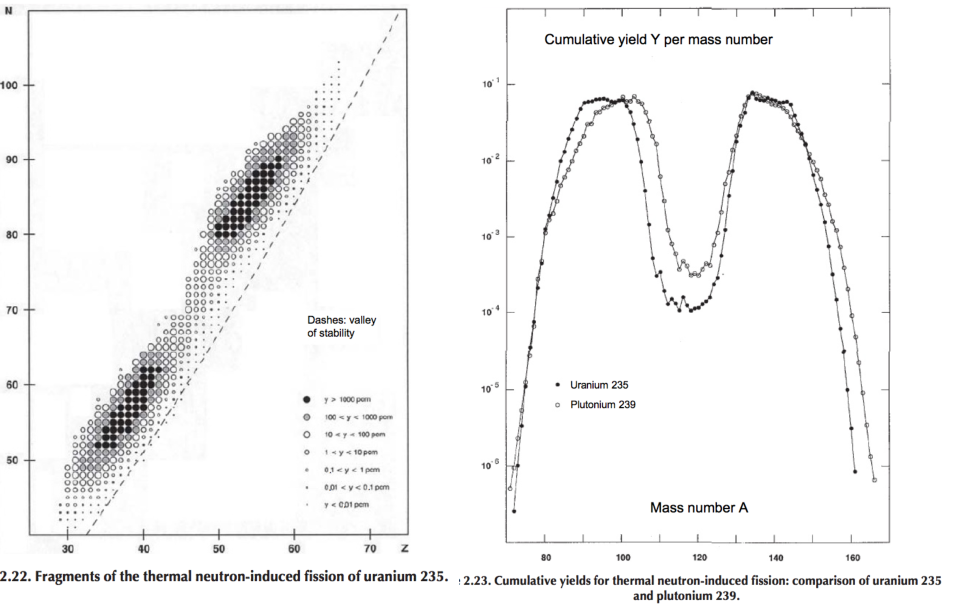
\includegraphics[width=5in]{images/dfs/fission-product-yield.png}
\end{figure}

\item Transient fission product equations: 
 \eqn{ \frac{\derivative N_i}{\dt} = \overbrace{\gamma_i \Sigma_f \phi}^{\mbox{fission production}} - \overbrace{\lambda_i N_i}^{\mbox{decay loss}} - \overbrace{\sigma_i N_i \phi}^{\mbox{loss by neutron capture}} }
\eqn{ + \overbrace{ \lambda_j N_j}^{\mbox{production of i by decay of j}} + \overbrace{\sigma_k N_k \phi}^{\mbox{production of i by neutron capture of k}} }
 Solving the above equation, we find that: 
 \begin{itemize}
   \item Equilibrium I-135 concentration is proportional to flux: $I_{eq} = \frac{\gamma_I \Sigma_f \phi}{\gamma_I}$;
   \item Equilibrium Xe-135 concentration depends on flux at low flux, and it is independent at high flux level: $X_{eq} = \frac{(\gamma_I + \gamma_X) \Sigma_f \phi}{\gamma_X + \sigma_X \phi}$;
   \item Equilibrium Pm-149 concentration is proportional to flux: $P_{eq} = \frac{\gamma \Sigma_f \phi}{\gamma}$;
   \item Equilibrium Sm-149 concentration is independent of flux: $S_{eq} = \frac{\gamma \Sigma_f}{\sigma}$. 
 \end{itemize}

\item I/Xe reactivity effects: Xe-135 has a thermal absorption cross section of $2.6\times 10^6$ barns. 
\begin{itemize}
\item Major source: Iodine decay; 
\item Major sink: burnup. 
\end{itemize}
Xenon peaking happens because after shutdown, the major sink is removed, but the major source remains, hence Xenon peaks until the Iodine depletes. Reactors must be designed with enough fuel to offset the effect of Xenon. At the end of core life, there may not be enough reactivity to override peak Xenon; such reactors are called `xenon-precluded.' If a scram occurs, a restart may not be possible for 30-40 hours. See Stacy's Example 6.2 (p.214) for an example of xenon reactivity worth and illustrating diagrams. 


\begin{table}
  \centering
  \begin{tabular}{|p{0.6\textwidth}|p{0.4\textwidth}|}\hline
    \begin{minipage}[b]{0.6\textwidth}
      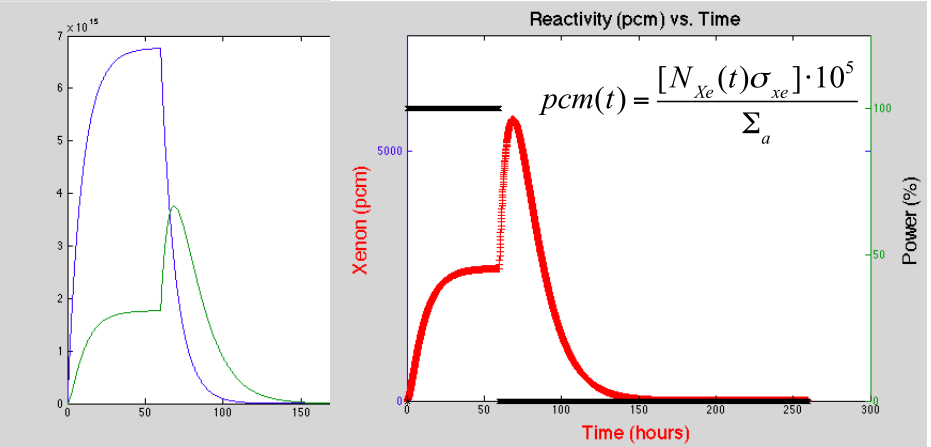
\includegraphics[width=3.5in]{images/dfs/I-Xe-1.png} 
    \end{minipage}
    & 
    \begin{minipage}[b]{0.4\textwidth}
      After startup: both I and Xe increases, and saturates after 30 hours. After shutdown: I decays quickly, whereas Xe peaks 9 hours after shutdown, and decays away in 60 hours. The peak happens because I coninues to decay into Xe, while Xe can no longer decrease through capture. 
There is a 2.5\% depress due to Xe; the higher the flux, the higher the peak is.
    \end{minipage}   \\ \hline
%
    \begin{minipage}[b]{0.6\textwidth}
      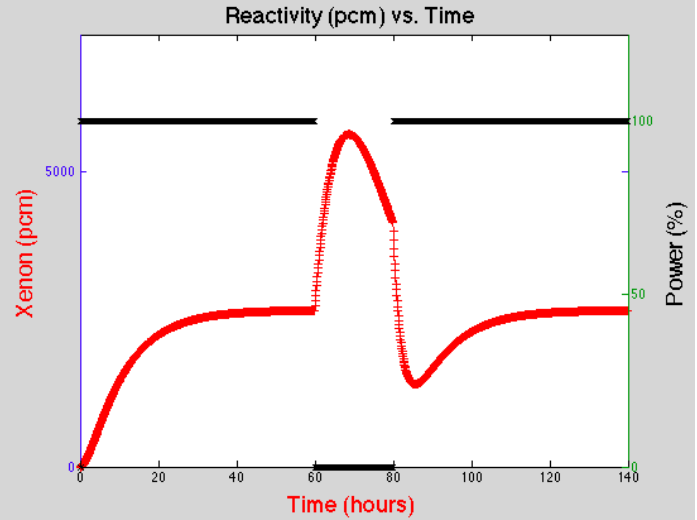
\includegraphics[width=3.5in]{images/dfs/I-Xe-2.png} 
    \end{minipage}
    & 
    \begin{minipage}[b]{0.4\textwidth}    
      A rapid startup after a scram: the concentration decreases immediately after the startup, because Xe absorption increases suddnely due to flux and the over-weight the amount from I decay. Xe would reach its equilibrium value again after about 40 hours. 
    \end{minipage}  \\ \hline
%
    \begin{minipage}[b]{0.6\textwidth}
      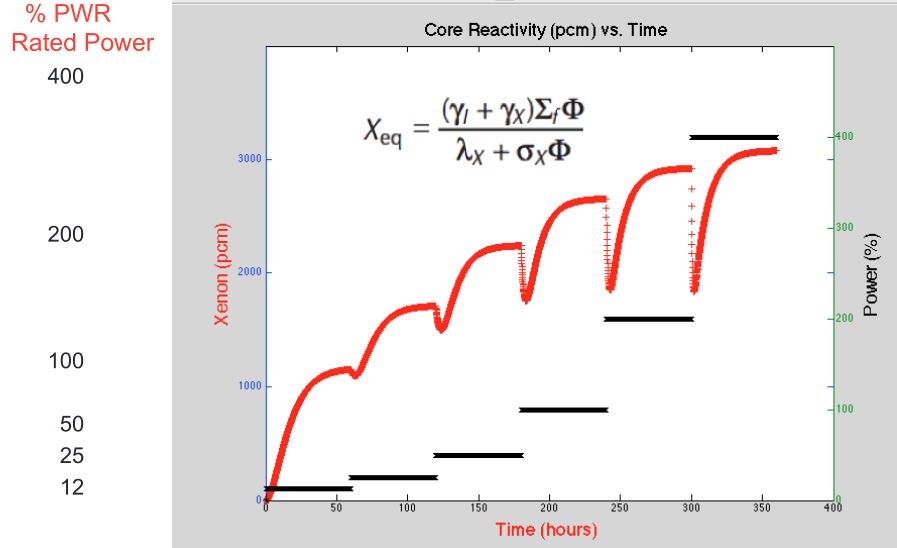
\includegraphics[width=3.5in]{images/dfs/I-Xe-3.png}
    \end{minipage}
 &  
    \begin{minipage}[b]{0.4\textwidth}    
      Equilibrium Xenon Worth: if $\phi \to \infty$, then $X_{eq}$ is independent of the flux as in the $X_{eq}$ expression; additionally, the Xenon concentration drops right after everytime power increases for the same reason as the previous case (flux increases, the destruction rate of Xe increases instantenously, but the Iodine decay rate has not increased yet). 
    \end{minipage} \\ \hline
%
    \begin{minipage}[b]{0.6\textwidth}
    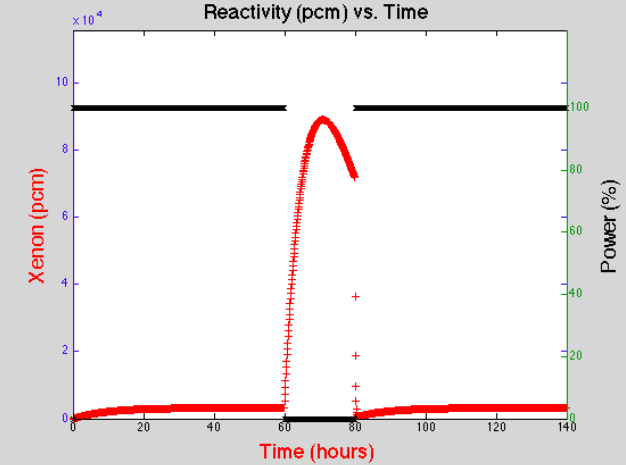
\includegraphics[width=3.5in]{images/dfs/I-Xe-4.png}
    \end{minipage}
 &  
    \begin{minipage}[b]{0.4\textwidth}
      Xenon for high flux reactor: xenon peak gives rise to a control constraint. If the reactivity reserves (control rods or poisons that can be removed) are insufficient, the reactor cannot be restarted during this period of increased xenon poisoning. We have to wait till Xe drops to re-start. Alternatively, you can start before Xenon builds up, which is pretty rare. 
      \end{minipage} \\ \hline
  \end{tabular}
\end{table}

\item  Pm/Sm reactivity effects: Samarium is another fission poisoner. It has one source: decay of Promethium; it has one sink: burnup. 

\begin{table}
  \centering
  \begin{tabular}{|p{0.6\textwidth}|p{0.4\textwidth}|}\hline
    \begin{minipage}[b]{0.6\textwidth}
      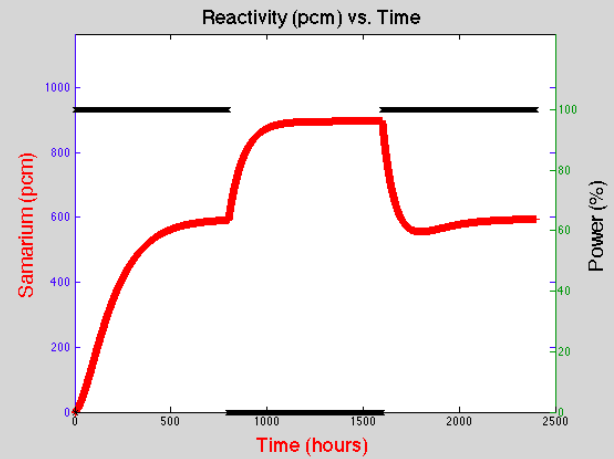
\includegraphics[width=3.5in]{images/dfs/Pm-Sm-1.png} 
    \end{minipage}
    & 
    \begin{minipage}[b]{0.4\textwidth}
      Promethium behaves normally: it builds up and reaches equilibrium when in operation, and it decays away after shutdown. 
Sm behaves similar to Xe in the sense that both peaks after reactor shutdown (Sm peaks 200 hours after shutdown, Xe peaks 9 hours after shutdown). But Sm is stable unlike Xe, and once Pm burns out, Sm would stay constant and never decay away. Sm reactivity peaks by 200-300 pcm after shutdown. 
    \end{minipage}   \\ \hline
%
    \begin{minipage}[b]{0.6\textwidth}
      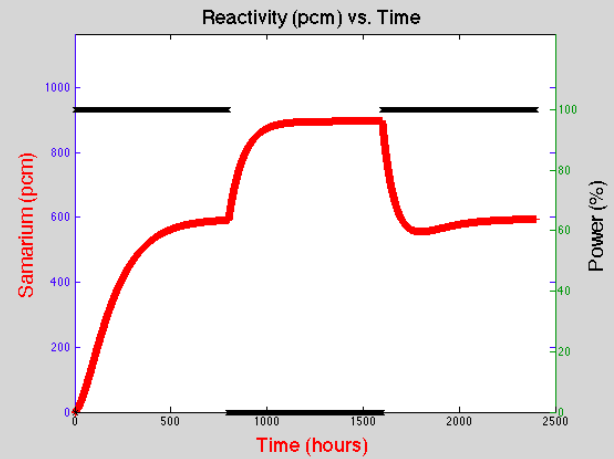
\includegraphics[width=3.5in]{images/dfs/Pm-Sm-2.png} 
    \end{minipage}
    & 
    \begin{minipage}[b]{0.4\textwidth}    
     Sm worth following a refueling outage: Over-write Xenon by pulling the control rods out for a couple of days; then insert the control rods for Sm. Sm returns to equilibrium about 100 hours after restart.
    \end{minipage}  \\ \hline
%
    \begin{minipage}[b]{0.6\textwidth}
      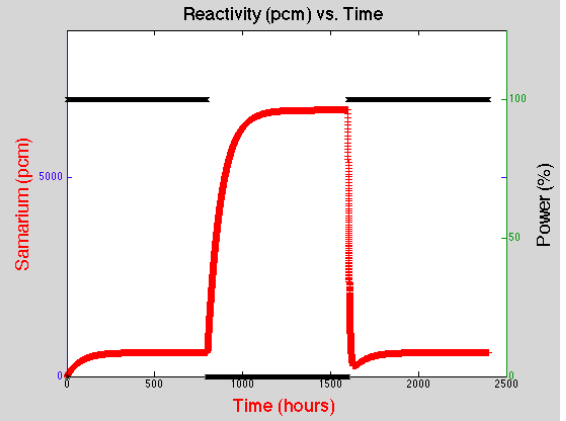
\includegraphics[width=3.5in]{images/dfs/Pm-Sm-3.png}
    \end{minipage}
    &  
    \begin{minipage}[b]{0.4\textwidth}    
      Sm for high flux reactor (20x PWR power density): Sm peaks a lot, which is bad because we may never be able to overrid Sm reactivity without refueling. Hence we should always have a controlled shutdown that burns out Xe/Sm before they build up. 
    \end{minipage} \\ \hline
  \end{tabular}
\end{table}
\end{enumerate}

\clearpage
\topic{Analytical Diffusion Theory} 
\begin{enumerate}
\item Transport cross section and diffusion coefficients: from the net current equation, assume the scattering is isotropic in the COM system, and use transport correction $P_0$ approximation, 
  \eqn{ D = \frac{1}{3 \Sigma_{tr} } }
  \eqn{ \Sigma_{tr} = \Sigma_t - \Sigma_{s1} = \Sigma_t - \frac{2}{3A} \Sigma_s }

\item Effective down-scattering cross section: 
  \eqn{ \hat{\Sigma}_{s12} = \bar{\Sigma}_{s12} - \bar{\Sigma}_{s21} \frac{\phi_2}{\phi_1} }
  So that up-scattering is zero: 
  \eqn{ \Sigma_{21}  = 0 }

\item Removal cross section
  \eqn{ \Sigma_{rg} = \Sigma_{tg} - \Sigma_{sgg} = \Sigma_{ag} + \Sum_{g'=1, g'\neq g}^G \Sigma_{sgg'}  }

\item Two-group diffusion equations,
  \begin{align}
    \left[ \begin{array}{cc} 
        \frac{\nu \bar{\Sigma}_{f1}}{\kinf} -  \bar{\Sigma}_{a1}  - \hat{\Sigma}_{s12} & \frac{\nu \bar{\Sigma}_{f2}}{\kinf}   \\
        \hat{\Sigma}_{s12} &  - \bar{\Sigma}_{a2}  
      \end{array} \right] 
    \left[ \begin{array}{c} \phi_1 \\ \phi_2 \end{array} \right] = 0
  \end{align}

\item Multi-group diffusion equations: See Section~\ref{multi-group-diffusion}. 
\begin{align}
& - \overbrace{\int_{E_g}^{E_{g-1}} \dE \divergence D(\vecr, E) \gradient \phi(\vecr, E)}^{\mbox{leakage/diffusion term }\textcircled{1}} + 
\overbrace{\int_{E_g}^{E_{g-1}} \dE \Sigma_t(\vecr, E) \phi(\vecr, E)}^{\mbox{total interaction term }\textcircled{2}} = \overbrace{\int_{E_g}^{E_{g-1}} \dE S(\vecr, E)}^{\mbox{source term } \textcircled{3}}  \\
& + \overbrace{\int_{E_g}^{E_{g-1}} \dE \chi(E) \int_{E'} \dE' \nu \Sigma_f (\vecr, E') \phi(\vecr, E')}^{\mbox{fission source term }\textcircled{4}} 
 + \overbrace{\int_{E_g}^{E_{g-1}} \dE \int_{E'} \dE' \Sigma_s(\vecr, E'\to E) \phi(\vecr, E')}^{\mbox{scattering source term }\textcircled{5}} 
\end{align}
\eqn{ -\divergence D_g(\vecr) \gradient \phi_g (\vecr) + \Sigma_{tg} (\vecr) \phi_g(\vecr) = \chi_g\Sum_{g'=1}^G \nu \Sigma_{fg'} \phi_{g'}(\vecr) + \Sum_{g'=1}^G \Sigma_{sg'g} (\vecr) \phi_{g'} (\vecr) + S_g(\vecr) }
Cancelling the within group scattering cross section from both sides and defining the group-wise removal cross section, we get the final form,
\eqn{ \boxed{- \divergence D_g(\vecr) \gradient \phi_g(\vecr) + \Sigma_{rg} (\vecr) \phi_g(\vecr) = \chi_g \Sum_{g'=1}^G \nu \Sigma_{fg'} (\vecr) \phi_{g'} (\vecr) + \Sum_{g'=1,g'\neq g}^G \Sigma_{sg'g} (\vecr) \phi_{g'} (\vecr) + S_g(\vecr) } }

\item Partial currents and albedos:
  \begin{align}
    J^+(\vecr, E) &= \int_{\vecn \cdot \vecOmega > 0} \vecn \cdot \vecOmega \psi(\vecr, E, \vecOmega) = \frac{1}{4\pi} \int_{\vecn \cdot \vecOmega > 0} \vecn \cdot \vecOmega [\phi(\vecr, E) + 3 \vecOmega \cdot \vecJ(\vecr, E) ] \\
    &= \frac{1}{4} \phi(\vecr, E) + \frac{1}{2} J_n (\vecr, E) \\
    J^-(\vecr, E) &= \int_{\vecn \cdot \vecOmega < 0} |\vecn \cdot \vecOmega| \psi(\vecr, E, \vecOmega)  \\
    &= \frac{1}{4} \phi(\vecr, E) - \frac{1}{2} J_n (\vecr, E) 
  \end{align}
  Albedo boundary condition is the measurement of how much flux is reflected back: 
  \eqn{ \alpha = \frac{J^- (\vecr_i, E)}{J^+ (\vecr_i, E)} }
  
\item Boundary conditions:
  \begin{enumerate}
  \item Zero flux boundary condition:
    \eqn{ \phi (0) = 0 }

  \item Zero incoming flux bc, integrating over all angles in half space, it is equivalent to zero incoming partial current:
    \eqn{ \left. \psi(\vecr, E, \vecOmega) \right|_{\vecn \cdot \vecOmega < 0} &= 0, & J^- (\vecr_i, E) &= 0}
    There are two formulism to solve this:
    \begin{itemize}
    \item Kord's formulism: 
      \eqn{ J^- (\vecr, E) &= \frac{1}{4} \phi(\vecr, E) - \frac{1}{2} J_n (\vecr, E)  = 0, & \Aboxed{ \frac{J}{\phi} &= \frac{1}{2} } }
    \item The more conventional approach is to approximate with extropolation boundary condition: 
      \begin{align}
        J^- &= \frac{1}{4} \phi + \frac{D}{2} \gradient \phi_n \\
        \Aboxed{ \frac{\gradient \phi}{\phi} &= - \frac{1}{2D} = - \frac{3\Sigma_{tr}}{2} = - \frac{1}{d_{\mathrm{extrap}}}} 
        \mbox{   where } d_{\mathrm{extrap}} = \frac{2}{3 \Sigma_{tr}}  = \frac{2}{3} \lambda_{\mathrm{tr}}
      \end{align}
      where $D$ is the property of the material inside, and $\lambda_{tr}$ is transport mean free path. The coefficient before $\lambda_{tr}$ can be 0.711 in other formulism. 
    \end{itemize}
  \end{enumerate}

\item Interface conditions: 
  \begin{enumerate}
    \item Continuity of scalar flux: 
      \eqn{ \phi(\vecr_i^-, E) = \phi(\vecr_i^+, E) }
    \item Continuity of normal current:
      \eqn{ \vecn \cdot D(\vecr_i^-, E) \gradient \phi(\vecr_i^-, E) = \vecn \cdot D(\vecr_i^+, E) \gradient \phi(\vecr_i^+, E) }
  \end{enumerate}
\end{enumerate}

\clearpage
\topic{Other Diffusion-Related Equations}
\begin{enumerate}
\item Balance equation derived from transport equations,
  \eqn{ \divergence \vecJ (\vecr, E) + \Sigma_t (\vecr, E) \phi(\vecr, E) = \Sum_i \int_{E'} \dE' \Sigma_s^i (\vecr, E'\to E) \phi(\vecr, E') + S_0 (\vecr, E) }
This expression is exact, because we haven't approximate $\vecJ$ yet. 

\item Using $P_1$ angular flux expansion,
  \eqn{ \psi (\vecr, E, \Omegahat) = \frac{1}{4\pi} \left[ \phi(\vecr, E) + 3 \Omegahat \cdot \vecJ(\vecr, E) \right] }
  We can get the net current equation,
  \eqn{ \frac{1}{3} \gradient \phi(\vecr, E) + \Sigma_t (\vecr, E) \vecJ(\vecr, E) = \Sum_i \int_{E'} \dE' \Sigma_{s1}^i (\vecr, E'\to E) \vecJ(\vecr, E') + \vec{S}_1(\vecr, E) }

\item From net current equation, assume no source and isotropic scattering in lab system, we can approximate the transport equation as, 
  \eqn{ \Sigma_{tr}^i (E) = \Sigma_t^i (E) - \frac{2}{3A^i} \Sigma_s^i (E) }
  Then we can solve for diffusion coefficient $D = \frac{1}{3 \Sigma_{tr}}$. 

\item One-group diffusion equation,
  \eqn{ -\divergence D(\vecr) \gradient \phi(\vecr) + \Sigma_a(\vecr) \phi(\vecr) = \frac{1}{\keff} \nu \Sigma_f(\vecr) \phi(\vecr) }

\item Helmoltz Equation: from one-group diffusion equation, we assume spatial constant cross section and use buckling term, 
  \eqn{ \laplacian \phi(\vecr) + B^2 \phi(\vecr) = 0 }
  This equation is important in showing that $\phi(\vecr)$ has a constant curvature. 
\end{enumerate}

\clearpage
\topic{Practise Problems}
\begin{enumerate}
\item Homogeneous (single-region) criticality problems:
  \begin{enumerate}
  \item 1D slab $\in  \left[- \frac{L_0}{2}, \frac{L_0}{2} \right]$, no source, critical. 
    \eqn{ \dphidxn2 + B^2 \phi (x) &= 0, &\phi(x) &= A \cos (Bx) + C \sin(Bx) }
    BCs: $\phi(\pm L/2) = 0$, where $\frac{L}{2} = \frac{L_0}{2} + 0.711 \lambda_{tr}$. Two equations two unknowns, 
    \eqn{ \left[ \begin{array}{cc} \cos(BL/2) & \sin(BL/2) \\ \cos(BL/2) & -\sin(BL/2) \end{array} \right] \left[ \begin{array}{cc} A \\ C \end{array} \right] = 0 }
    Set the determinant to be zero, we get $-2 \cos (BL/2) \sin (BL/2) = 0$. There are two possibilities: 
    \eqn{ B_n&= \frac{n\pi}{L}  & \phi(x) &= \left\{ 
      \begin{array}{cc} 
        A_n \cos (B_n x) & n=1,3,5, \cdots \\
        A_n \sin (B_n x) & n=2,4,6, \cdots 
      \end{array} \right. }
    But in order for $\phi(x) \ge 0$ everywhere, only $n=1$ is possible; that is, 
    \eqn{ \phi(x) = A \cos \frac{\pi x}{L} }
    and the criticality condition implies that, 
    \eqn{ \frac{\nu \Sigma_f - \Sigma_a}{D}  = \left( \frac{\pi}{L} \right)^2 }

  \item Find the height-to-diameter that would minimize the leakage from a fixed-volume cylinder. To minimize leakage, we need to maximize $B_m^2$ hence $B_g^2$. For a finite cylinder, we know
    \eqn{B_g^2 = \left( \frac{2.405}{R} \right)^2 + \left( \frac{\pi}{H} \right)^2 }
    and we solve $\frac{\derivative B_g^2}{\dr} = 0$. The optimal H/D ratio comes out to be 0.9236. 
    
  \end{enumerate}
  Summary: only the lowest node remains after the source is gone. For any positive value of material buckling, there is a unique critical size for each geometry. 
  
\item Homogeneous (single-region) source problems:
  \begin{enumerate}
  \item See Section~\ref{one-group-source-problem-subcritical}
  \item 
  \end{enumerate}
  
\item Multi-region diffusion problems
\end{enumerate}

\clearpage
\topic{Numerical Diffusion Theory}
\begin{enumerate}
\item Finite-difference diffusion equation: 
\begin{align*}
 - \hat{D}_1^{n-1,n} \phi_1^{n-1} - \hat{D}_1^{n,n+1} \phi_1^{n+1} + [ \Sigma_{r1}^n \Delta^n + \hat{D}_1^{n-1, n} + \hat{D}_1^{n,n+1} ] \phi_1^n 
&= \nu \Sigma_{f1}^n \phi_1^n \Delta^n + \nu \Sigma_{f2}^n \phi_2^n \Delta^n + S_1^n \Delta^n \\
- \hat{D}_2^{n-1,n} \phi_2^{n-1} - \hat{D}_2^{n,n+1} \phi_2^{n+1} + [\Sigma_{a2}^n \Delta^n + \hat{D}_2^{n-1.n} + \hat{D}_2^{n,n+1} ] \phi_2^n 
&= \Sigma_{s12}^n \phi_1^n \Delta^n + S_2^n \Delta^n 
\end{align*}

\item Fission source iterations: the equation we are trying to solve is,
\eqn{ [A] [\phi]^{n+1} &= [M] [\phi]^n }
An initial guess of the flux $\phi_i^{(0)}$ at each point and of the eigenvalue $\lambda^{(0)}$ is made and an initial fission source at each point is constructed $S_i^{(0)} = M \phi_i^{(0)}$. The Gaussian elimination is performed to determine $\phi_i^{(1)} = A^{-1} S_i^{(0)}$. Then we update the source term as well based on the flux. A new estimate of the eigenvalue is made from: 
\eqn{ \keff = \frac{S_i^{(1)}}{S_i^{(0)}} }
The process is continued until the eigenvalues obtained on two successive iterates differ by less than a threshold level. The rate our fission source converges depends on material, geometry etc.

\item Gauss-Jacobi flux inner iterations: 
\begin{figure}[ht]
  \centering
  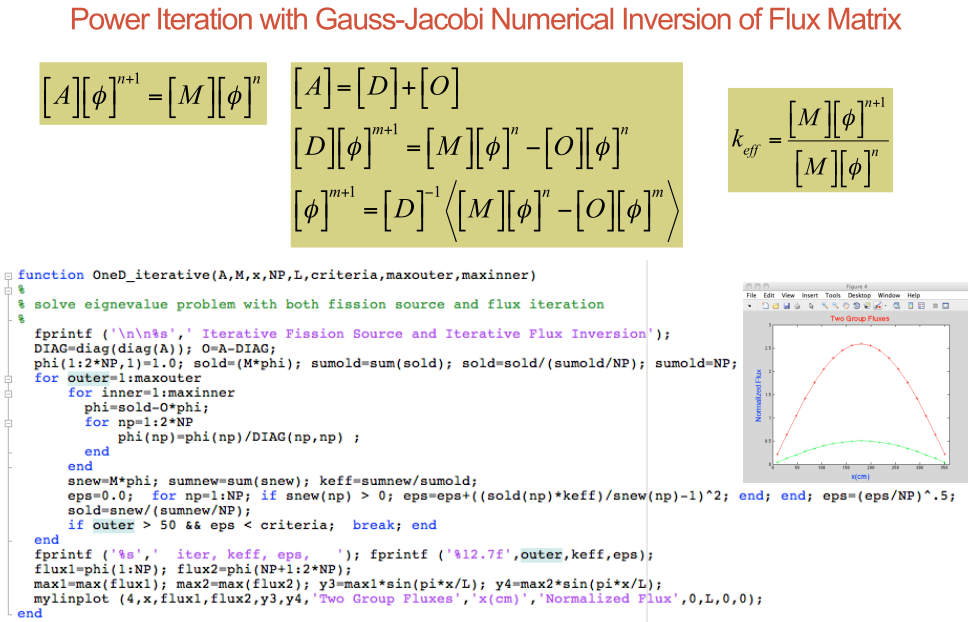
\includegraphics[width=4in]{images/dfs/power-iteration-Gauss-Jacobi.png}
\end{figure}

\item Dominance ratio estimation: 
Given an eigenvalue problem, if we specify the solved eigenvalues to be:
\eqn{ |\lambda_1| > |\lambda_2| \ge |\lambda_3| \ge \cdots }
then $|\lambda_1|$ is the spectral radius of the iteration matrix, and every mode has a dominance ratio,
\eqn{ \dr_n = \frac{\lambda_n}{\lambda_1} }
and power iteration kills of the lowest dominance ratio modes. The last remaining mode is the fundamental mode $dr = \frac{\lambda_2}{\lambda_1}$. If $|\lambda_1| \ge 1$, the ietration scheme is unstable and it would not converge. Convergence of the power method is slow when $d$ is close to unity; in fact in most numerical methods, convergence rate = 1 - dominance ratio.

Dominance ratio measures the spatial decoupling, and it depends on: symmetric mode, core size, decoupling of the radial zones, and of the axial zones. 
\end{enumerate}


\end{document}
